\section{Froehlich polaron: Feynman diagrams}
In order to deeply understand a many-body system such as the Froehlich polaron it is necessary to use a more powerful formalism 
derived from quantum field theory, we will first breafly describe Green's functions as an effective mean to describe meaningful quantities of 
our system and we will then shift to the \textbf{Matsubara imaginary time} formalism, much more useful in the context of Diagrammatic Monte Carlo.
At the end of this journey the connection between the Froehlich polaron and Feynman diagrams will be explicated. In this section of the thesis 
we will use the convention $\hbar=1$.
\subsection{Green's function formalism}
Green functions are useful objects to perturbatively solve systems that are really hard to correctly treat in any other way \cite{bruus2004many}.\\
If we take for example a time-dependent Schroedinger equation in the following way:
\begin{equation}
    \left[i\partial_t - H_0(\mathbf{r})-V(\mathbf{r})\right]\psi(\mathbf{r},t)=0,
    \label{Schroedinger_eq_hamiltonian}
\end{equation}
with the non-interacting diagonizable term $H_0$ and the perturbation $V$. It is possible to define the corresponding Green's functions as:
\begin{equation}
\begin{split}
    \left[i\partial_t -H_0(\mathbf{r})\right]G_0(\mathbf{r},\mathbf{r}';t,t')&=\delta(\mathbf{r}-\mathbf{r}')\delta(t-t'),\\
    \left[i\partial_t -H_0(\mathbf{r})-V(\mathbf{r})\right]G(\mathbf{r},\mathbf{r}';t,t')&=\delta(\mathbf{r}-\mathbf{r}')\delta(t-t').
\end{split}
    %\left[E-H_0(\mathbf{r})\right]G_0(\mathbf{r},\mathbf{r}',E)=\delta(\mathbf{r}-\mathbf{r'}),\hspace{0.5cm}with\hspace{0.5cm}G_0(\mathbf{r},\mathbf{r}')=G_0(\mathbf{r}',\mathbf{r}).
\end{equation}
We can define $G_0^{-1}(\mathbf{r};t')$ and $G^{-1}(\mathbf{r};t)$ as:
\begin{equation}
\begin{split}
    &G_0^{-1}(\mathbf{r};t)=i\partial_t-H_0(\mathbf{r}),\\
    &G^{-1}(\mathbf{r};t)=i\partial_t-H_0(\mathbf{r})-V(\mathbf{r}),
\end{split}
\label{GF_solving_eq}
\end{equation}
%and thus
%\begin{equation}
%    G_0^{-1}(\mathbf{r},E)G_0(\mathbf{r},\mathbf{r}',E)=\delta(\mathbf{r},\mathbf{r}').
%\end{equation}
The Schroedinger equation can then be recast as
\begin{equation}
    \left[G^{-1}_0(\mathbf{r},t)-V(\mathbf{r})\right]\psi(\mathbf{r},t)=0
\end{equation}
and it is possible to rewrite the system as an integral equation
\begin{equation}
    \psi(\mathbf{r},t)=\psi^0(\mathbf{r},t)+\int d^3r'\int dt' G_0(\mathbf{r},\mathbf{r}';t,t')V(\mathbf{r}')\psi(\mathbf{r}',t')
    \label{GF_expansion_integral}
\end{equation}
which can be solved iteratively. In fact:
\begin{equation}
\begin{split}
    %\psi_E(\mathbf{r})=\psi^0_E(\mathbf{r})+\int d^3 r'G_0(\mathbf{r},\mathbf{r}',E)V(\mathbf{r}')\psi_E^0(\mathbf{r}')+O(V^2).
    \psi&= \psi^0+G_0V\psi^0+G_0VG_0V\psi^0+G_0VG_0VG_0V\psi^0+...\\
    &= \psi^0+(G_0+G_0VG_0+G_0VG_0VG_0+...)V\psi_0.
\end{split}
\label{expansion_G}
\end{equation}
Noting that \ref{GF_expansion_integral} can be also written as:
\begin{equation}
    \psi(\mathbf{r},t)=\psi^0(\mathbf{r},t)+\int d^3r'\int dt' G(\mathbf{r},\mathbf{r}';t,t')V(\mathbf{r}')\psi^0(\mathbf{r}',t'),
\end{equation}
it is possible to identify $G$ with
\begin{equation}
\begin{split}
    G&=G_0+G_0VG_0+G_0VG_0VG_0+...\\
    &=G_0+G_0V(G_0+G_0VG_0+...),
\end{split}
\end{equation}
and the well-known \textbf{Dyson equation} is retrieved:
\begin{equation}
    G=G_0+G_0VG.
    \label{Dyson_Eq}
\end{equation}
The one described above is the \textbf{single particle Green's function}, also called propagator since it "propagates" the wavefunction: in fact,
if the wavefunction is known at time $t'$ the wavefunction at a later time can be obtained in the following way:
\begin{equation}
    \psi(\mathbf{r},t)=\int d^3r'\int dt' G(\mathbf{r}t,\mathbf{r}'t')\psi(\mathbf{r}'t'),
\end{equation}
which is a solution to \ref{GF_solving_eq}.
The Green's function can also be written as
\begin{equation}
    G(\mathbf{r}t,\mathbf{r}'t')=-\theta(t-t')\langle \mathbf{r}|e^{-iH(t-t')}|\mathbf{r}'\rangle,
\end{equation}
and is more precisely known as the \textbf{retarded Green's function}.\\
Focusing now on a many-body system the Green's function is defined as
\begin{equation}
    G^R(\mathbf{r}\sigma t,\mathbf{r}'\sigma't')=-i\theta(t-t')\langle[\psi_\sigma(\mathbf{r},t),\psi^\dagger_{\sigma'}(\mathbf{r}',t')]_{B,F}\rangle,
\end{equation}
where $[,]_{B,F}$ is the commutator $[,]$ for bosons and the anticommutator $\{,\}$ for fermions.\\
In the case of translation-invariant system (such as lattices) Green's functions can only depend on $\mathbf{r}-\mathbf{r}'$ and 
it is natural to adopt the usual $\mathbf{k}$ formalism:
\begin{equation}
\begin{split}
    G^R(\mathbf{r}-\mathbf{r}',\sigma t,\sigma' t')&=\frac{1}{V}\sum_\mathbf{k}e^{i\mathbf{k}\cdot(\mathbf{r}-\mathbf{r}')}G^R(\mathbf{k},\sigma t,\sigma' t'),\\
    G^R(\mathbf{k},\sigma t,\sigma' t')&=-i\theta (t-t')\langle [a_{\mathbf{k}\sigma},a^\dagger_{\mathbf{k}'\sigma'}]_{B,F}\rangle.
\end{split}
    \label{GF_momentum_space}
\end{equation}
The goal is now to find explicit expressions for the various Green's function of relevance, in the special case of a free electron 
the Hamiltonian assumes the simple form
\begin{equation}
    H=\sum_{\mathbf{k}\sigma}\epsilon(k)c^\dagger_{\mathbf{k}\sigma}c_{\mathbf{k}\sigma}, 
\end{equation}
and the time dependence of the creation/annihilation operators is simply defined as
\begin{equation}
    c_{\mathbf{k}\sigma}(t)=e^{iHt}c_{\mathbf{k}\sigma}e^{-iHt}=c_{\mathbf{k}\sigma}e^{-i\xi_kt}.
\end{equation}
The retarded Green's function then becomes:
\begin{equation}
    G^R(\mathbf{k}\sigma,t-t')=-i\theta(t-t')e^{-i\xi_k(t-t')}.
\end{equation}
\subsection{Perturbation theory for Green's functions}
Given an Hamiltonian which can be written as a sum of two terms
\begin{equation}
    H=H_0+V,
    \label{interacting-form-Hamiltonian}
\end{equation}
where $H_0$ is diagonizable and $V$ is an interaction term which can be treated perturbatively, we want to obtain a perturbative expansion 
of the Green's function. The issue with this approach is that in the expression for a generic Green's function it is require to take the expectation value  
over a ground state $(\langle \cdot \rangle)$ which is not known, namely the ground state of the interacting system.\\
It is thus important to link the ground state of the interacting system to the ground state of the non-interacting one, to this mean we 
introduce \textbf{adiabatic switching on of the interaction} \cite{nolting2009fundamentals}.\\
The core feature of this method is turning a time-independent problem into a time-dependent one by slowly switching on the perturbation, the Hamiltonian 
is transformed in the following way:
\begin{equation}
    H_\alpha(t)=H_0+Ve^{-\alpha|t|},\hspace{1cm}\alpha>0,
\end{equation}
such that the system is non-interacting for $t\to\pm\infty$ and goes back to \ref{interacting-form-Hamiltonian} for $t\to\infty$,
\begin{equation}
    \lim_{t\to\pm\infty}H_\alpha(t)=H_0,\hspace{1cm}\lim_{t\to 0}H_\alpha(t)=H.
\end{equation}
In this setup, it is natural to suppose that the ground state of the interacting system $|\Phi_0\rangle$ evolves continuously starting from 
the ground state of the non-interacting one $|\Psi_0\rangle$.\\
We introduce the Dirac representation the operators, for the interaction term of the Hamiltonian we have
\begin{equation}
    V_{I}e^{-\alpha |t|} = e^{iH_0t}Ve^{-iH_0t}e^{-\alpha|t|},
\end{equation}
the time-evolution operator in the Dirac representation is written as
\begin{equation}
    U_{I\alpha}(t,t_0)=\sum_{n_0}^\infty \frac{1}{n!}(-i)^n \int_{t_0}^t dt_1\cdots\int_{t_0}^t dt_n e^{-\alpha(|t_1|+...+|t_n|)}T_t\left[V_I(t_1)\cdots V_I(t_n)\right],
    \label{t-evolution-perturbatively}
\end{equation}
and defines the evolution of the system in the following way:
\begin{equation}
    |\psi_{I\alpha}(t)\rangle=U_{I\alpha}(t,t_0)|\psi_{I\alpha}(t_0)\rangle.
\end{equation}
The equation of motion is obtained as
\begin{equation}
    i\frac{d}{dt}|\psi_{I\alpha}(t)\rangle = e^{-\alpha |t|} V_I(t)|\psi_{I\alpha}(t)\rangle,
\end{equation}
from this it follows that 
\begin{equation}
    i\frac{d}{dt}|\psi_{I\alpha}(t\pm\infty)\rangle = 0,
\end{equation}
which means that the state is time-independent. We can thus take the ground state of the non-interacting system as the ground state for the 
interacting system when $t\to\pm\infty$, the expression at the two times can differ up to a phase factor:
\begin{equation}
    |\psi_{I\alpha}(t\to-\infty)\rangle=|\Psi_0\rangle,\hspace{1cm}|\psi_{I\alpha}(t\to\infty)\rangle=e^{i\phi}|\Psi_0\rangle.
\end{equation}
It is now possible to link the non-interacting ground state at $t\to-\infty$ with the interacting one at $t$ using the time-evolution 
operator
\begin{equation}
    |\psi_{I\alpha}(t)\rangle=U_I(t,-\infty)|\Psi_0\rangle,
\end{equation}
at $t=0$ the interaction is completely switched on. Moreover, if the switching on is performed really slowly (adiabatically) it can be 
excluded that the wavefunction $|\psi_{I\alpha}(t)$ depends on the parameter $\alpha$ and the exact ground state should be computed starting from 
the non-interacting ground state.\\
However, since it is required that $\alpha>0$, there is no certainty that the limit
\begin{equation}
    |\Phi_0\rangle=\lim_{\alpha\to0}|\psi_{I\alpha}(0)\rangle
\end{equation}
exists, and in fact it does not exist.\\
For this reason the \textbf{Gell-Mann-Low theorem} \cite{PhysRev.84.350} is used, which is a theorem that fixes the eigenstate which evolves from the non-interacting 
ground state during the adiabatic switching on of the interaction.\\
The statement of the theorem is the following: given a state
\begin{equation}
    \lim_{\alpha\to 0}\frac{U_{I\alpha}(0,-\infty)|\Psi_0\rangle}{\langle\Psi_0|U_{I\alpha,-\infty}|\Psi_0\rangle}=\lim_{\alpha\to 0}\frac{|\psi_{I\alpha}(0)\rangle}{\langle\Psi_0|\psi_{I\alpha}(0)\rangle}
\end{equation}
which exists for every order of the perturbation theory, then this state is an eigenstate $|\Phi_0\rangle$ of the full Hamiltonian $H_0$.\\
The importance of this system consists on the fact that it fixes the eigenstate during its evolution starting from the non-interacting ground 
state, a further important assumption is thus the requirement that no crossings of the states occur during their evolution from the free states. This is not 
a problem in our case since in the Froehlich Hamiltonian no transitions of this type occur, differently from what happens, for example, 
in superconductivity.\\
Since Green's functions are defined as expectation values of Heisenberg operators, these expectation values should be evaluated over the ground state (at $T=0$), 
Using Gell-Mann-Low theorem it was demonstrated that the ground state of the interacting system $|\Phi_0\rangle$ can be retrieved from the non interacting one $|\Psi_0\rangle$, 
the normalized ground state is
\begin{equation}
    |\Phi_0\rangle_{norm}=\frac{|\Phi_0\rangle}{\left(\langle \Phi_0|\Phi_0\rangle\right)^{1/2}}.
\end{equation}
Given a generic Green's function (in terms of the parameter $\alpha$)
\begin{equation}
    G_\alpha(\mathbf{k}t,\mathbf{k}'t')=-i\langle T_t c_{\mathbf{k}}(t)c^\dagger_{\mathbf{k}'}(t')\rangle,
\end{equation}
the creation and annihilation operators in the Heisenberg representation can be cast in the interaction one:
\begin{equation}
    c_{\alpha\mathbf{k}}(t)=U_{I\alpha}(0,t)c_{I\alpha\mathbf{k}}(t)U_{I\alpha}(t,0).
\end{equation}
The expectation value of the Heisenberg operator can now be computed:
\begin{equation}
\begin{split}
    &_{norm}\langle \Psi_0|c_{\mathbf{k}}(t)c^\dagger_{\mathbf{k}'}(t')|\Psi_0\rangle_{norm}=\frac{\langle\Psi_0|c_{\alpha\to0\mathbf{k}}c^\dagger_{\alpha\to0\mathbf{k}'}|\Psi_0\rangle}{\langle\Psi_0|\Psi_0\rangle}\\
    &=\lim_{\alpha\to0}\frac{\langle\Psi_0|U_{I\alpha}(+\infty,t)c_{I\mathbf{k}}(t)U_{I\alpha}(t,t')c^\dagger_{I\mathbf{k}'}(t')U_{I\alpha}(t',-\infty)|\Psi_0\rangle}{\langle\Psi_0|U_{I\alpha}(+\infty,-\infty)|\Psi_0\rangle}.
\end{split}
\end{equation}
Using this formula it is possible to perturbatively treat any Green's function by expanding it in a power series.\\
Given a generic Heisenberg operator $A(t)$ and the power expansion for the time-evolution operator in \ref{t-evolution-perturbatively} we may write:
\begin{equation}
\begin{split}
    &_{norm}\langle \Psi_0|A(t)|\Psi_0\rangle_{norm}=\lim_{\alpha\to 0}\frac{1}{\langle \Psi_0|U_{I\alpha}(+\infty,-\infty)|\Psi_0\rangle}\sum_{n=0}^{+\infty}\frac{1}{n!}\left(-i\right)^n\cdot \\
    &\int_{-\infty}^{+\infty}dt_1\cdots\int_{-\infty}^{+\infty}dt_n e^{-\alpha(|t_1|+...+|t_n|)}\langle\Psi_0|T\left(V_I(t_1)\cdots V_I(t_n)\right)|\Psi_0\rangle.
\end{split}
\label{expansion_expectation_value}
\end{equation}
It is then possible to compare \ref{expansion_expectation_value} with \ref{t-evolution-perturbatively} to obtain the following identity:
\begin{equation}
\begin{split}
    \sum_{n=0}^{+\infty}\frac{1}{n!}(-i)^n\int_{-\infty}^{+\infty}&dt_1\cdots\int_{-\infty}^{+\infty}dt_ne^{-\alpha(|t_1|+...+|t_n|)}T_t\left(V_I(t_1)\cdots V_I(t_n)A(t)\right)=\\
    =&U_{I\alpha}(+\infty,t)A(t)U_{I\alpha}(t,-\infty).
\end{split}
\end{equation}
The same argument can be made for a single particle Green's function, obtaining a similar expansion:
\begin{equation}
\begin{split}
    iG(\mathbf{k},t,t')=\sum_{n=0}^{+\infty}&\frac{1}{n!}(-i)^n\int_{-\infty}^{+\infty}dt_1\cdots\int_{-\infty}^{+\infty}dt_n\cdot \\
    &e^{-\alpha(|t_1|+...+|t_n|)}\langle\Psi_0|T_t\left(V_I(t_1)\cdots V_I(t_n)c_\mathbf{k}(t)c^\dagger_{\mathbf{k}}(t')\right)|\Psi_0\rangle.
\end{split}
\end{equation}
\subsection{Matsubara formalism for imaginary time Green's functions}
The usual Green's functions are complex objects that are not fit to be used in the Diagrammatic Monte Carlo method since they provides 
negative values that cannot be easily sampled from a distribution without losing precision.\\
For this reason we now describe the imaginary time formalism for Green's functions, which is also useful to evaluate system that are 
at non-zero temperature. The relevant substitution is:
\begin{equation}
    it\to \tau,
    \label{imaginary_time_substitution}
\end{equation}
%it is important to stress that this imaginary time formalism does not have any physical meaning and is just an useful mathematical framework.\\
the retarded Green's function previously defined in \ref{GF_momentum_space} thus becomes the following Matsubara Green's function:
\begin{equation}
    G(\mathbf{k},\sigma\tau,\sigma'\tau')=-\theta(\tau-\tau')\langle [a_{\mathbf{k}\sigma},a^\dagger_{\mathbf{k}'\sigma'}]_{B,F}\rangle
\end{equation}
where the thermal average $\langle A(\tau)B(\tau')\rangle$ is defined as:
\begin{equation}
\begin{split}
    &\langle \Psi_0|A(\tau)B(\tau')|\Psi_0\rangle\hspace{1.75cm}T=0,\\
    &\frac{1}{Z}Tr\left[e^{-\beta H}A(\tau)B(\tau')\right]\hspace{0.8cm}T>0.
\end{split}
\end{equation}
where $\Psi_0$ is the ground state and $Z$ the partition function.\\
Given a system with a Hamiltonian characterized by a diagonizable term $H_0$ and a perturbation $V(\tau)$, we can define the imaginary time 
Heisenberg picture for an operator $A$ as 
\begin{equation}
    A(\tau)=e^{-\tau H}Ae^{\tau H},
\end{equation}
and similarly the imaginary time interaction picture as
\begin{equation}
    A_I(\tau)=e^{\tau H_0}Ae^{-\tau H_0}.
\end{equation}
We can define the imaginary time time-evolution operator in the interaction picture as 
\begin{equation}
    U_I(\tau,\tau')=e^{\tau H_0}e^{-(\tau-\tau')H}e^{-\tau'H_0},
\end{equation}
an explicit expression for the interaction picture time-evolution operator in the imaginary time formalism is found in analogy with 
the real time counterpart
\begin{equation}
    \frac{\partial}{\partial\tau} U_I(\tau,\tau')=e^{\tau H_0}(H_0-H)e^{-(\tau-\tau')H}e^{-\tau'H_0}=-V_I(\tau)U_I(\tau,\tau'),
\end{equation}
which can be solved iteratively:
\begin{equation}
\begin{split}
    U_I(\tau,\tau')&=\sum_{n=0}^\infty\frac{1}{n!}(-1)^n\int_{\tau'}^{\tau}d\tau_1...\int{\tau'}^{\tau}d\tau_nT_\tau\left[V_I(\tau_1)...V_I(\tau_n)\right]\\
    &=T_\tau\exp{\left(-\int_{\tau'}^\tau d\tau_1V_I(\tau_1)\right)},
\end{split}
\end{equation}
where $T_\tau$ is the $\tau$ ordering operator.\\
It is also important to stress that the partition function $Z$ is naturally treated in the imaginary time formalism, in fact:
\begin{equation}
    e^{-\beta H}=e^{-\beta H_0}U_I(\beta,0)=e^{-\beta H_0}T_\tau exp{\left(-\int_{0}^{\beta}d\tau_1V_I(\tau_1)\right)},
\end{equation}
and we have
\begin{equation}
\begin{split}
    \langle T_\tau A(\tau)B(\tau')\rangle &= \frac{1}{Z}Tr\left[e^{-\beta H}T_\tau(A(\tau)B(\tau'))\right]\\
    &=\frac{1}{Z}Tr\left[e^{-\beta H_0}U_I(\beta,0)T_\tau(U_I(0,\tau)A_I(\tau)U_I(\tau,\tau')B_I(\tau')U_I(\tau',0)) \right]\\
    &=\frac{1}{Z}Tr\left[e^{-\beta H_0}T_\tau(U_I(\beta,0)A_I(\tau)B_I(\tau'))\right]\\
    &=\frac{\langle T_\tau U_I(\beta,0)A_I(\tau)B_I(\tau')\rangle_0}{\langle U_I(\beta,0)\rangle_0},
\end{split}
\end{equation}
where the expectation value is taken on the non-interacting system, in agreement with the previously found result for $T=0$.\\
We now go back to the definition of single particle Green's functions in imaginary time formalism, we can define them both in real space 
and in $\mathbf{k}$ space:
\begin{equation}
\begin{split}
    &G(\mathbf{r}t,\mathbf{r}'t')=-\langle T_\tau\left(\psi(\mathbf{r},\tau),\psi^\dagger(\mathbf{r}',\tau')\right)\rangle,\\
    &G(\mathbf{k}\tau,\mathbf{k}'\tau')=-\langle T_\tau\left(c_{\mathbf{k}}(\tau)c^\dagger_{\mathbf{k}'}(\tau')\right)\rangle,
\end{split}
\end{equation}
neglecting the spin $\sigma$ degree of freedom (not relevant for our treatment).\\
In the non-interacting case the Matsubara single particle Green's functions can be valued in the same way as the retarded Green's functions, 
in fact:
\begin{equation}
    H_0=\sum_{\mathbf{k}}\xi_\mathbf{k}c^\dagger_\mathbf{k}c_\mathbf{k},
\end{equation}
and the creation/annihilation operators in the Heisenberg picture read
\begin{equation}
    c_\mathbf{k}(\tau)=e^{\tau H_0}c_\mathbf{k}e^{-\tau H_0}=c_\mathbf{k}e^{-\xi_\mathbf{k}\tau},\hspace{1cm}c^\dagger_\mathbf{k}(\tau)=e^{\tau H_0}c^\dagger_\mathbf{k}e^{-\tau H_0}=c^\dagger_\mathbf{k}e^{\xi_\mathbf{k}\tau}.
\end{equation}
The non-interacting Matsubara Green's function is then defined as 
\begin{equation}
\begin{split}
    G_0(\mathbf{k},\tau,\tau')&=-\langle T_\tau\left(c_\mathbf{k}(\tau)c^\dagger_\mathbf{k}(\tau')\right)\rangle\\
    &=-\theta(\tau-\tau')\langle c_\mathbf{k}(\tau)c^\dagger_\mathbf{k}(\tau')\rangle-(\pm)_{B,F}\theta(\tau'-\tau)\langle c^\dagger_\mathbf{k}(\tau')c_\mathbf{k}(\tau)\rangle\\
    &=-\left[\theta(\tau-\tau')\langle c_\mathbf{k}c^\dagger_\mathbf{k}\rangle-(\pm)_{B,F}\theta(\tau'-\tau)\langle c_\mathbf{k}^\dagger c_\mathbf{k}\rangle\right]e^{-\xi_\mathbf{k}(\tau-\tau')}.
    \label{free_propagator}
\end{split}
\end{equation}
\subsection{Equation of motion and Wick's theorem}
For a general Green's function the process to find its expression goes through the equation of motion technique, for a general 
operator in the imaginary time formalism the time derivative is
\begin{equation}
    \partial_\tau A(\tau)= \partial(\tau)\left(e^{\tau H}Ae^{-\tau H}\right)=e^{\tau H}[H,A]e^{-\tau H}=[H,A](\tau),
\end{equation}
if we derivate with respect to imaginary time a Matsubara Green's function the following result is obtained:
\begin{equation}
    -\frac{\partial}{\partial\tau}\left(T_\tau\langle A(\tau)B(\tau')\rangle\right)=\delta(\tau-\tau')\langle(AB-(\pm)_{B,F}BA\rangle)+\langle T_\tau\left([H,A](\tau)B(\tau')\right)\rangle,
\end{equation}
which for the single particle Green's function in momentum space becomes
\begin{equation}
    -\frac{\partial}{\partial \tau} G(\mathbf{k}\tau,\mathbf{k}'\tau')=\delta(\tau-\tau')\delta_{\mathbf{k}\mathbf{k}'}+\langle T_\tau\left([H,c_\mathbf{k}](\tau)c^\dagger_{\mathbf{k}'}(\tau')\right)\rangle.
\end{equation}
In the case of a Green's function for a non-interacting system $G_0$ with an Hamiltonian $H_0=\sum_{\mathbf{kk}'}t_{\mathbf{kk}'}c^\dagger_\mathbf{k}c_{\mathbf{k}'}$ this equation simplifies to
\begin{equation}
    -\frac{\partial}{\partial\tau}G_0(\mathbf{k}\tau,\mathbf{k}'\tau')=\delta(\tau-\tau')\delta_{\mathbf{k}\mathbf{k}'}+\sum_{\mathbf{k}''}t_{\mathbf{kk}''}G_0(\mathbf{k}''\tau,\mathbf{k}'\tau'),
\end{equation}
and the solution is found as previously defined.\\
We now introduce \textbf{Wick's theorem}, an important result which states that higher order (greater than 1) Green's functions for non-interacting 
systems $G_0^{(n)}$ can be factorized into products of single particle Green's functions $G_0$.\\
The $n$-particle Green's function is defined as:
\begin{equation}
    G_0^{(n)}(\nu_1\tau_1,\cdots,\nu_n\tau_n;\nu_1'\tau_1',\cdots\nu_n'\tau_n')=(-1)^n\langle T_\tau \left[c_{I\nu_1}(\tau_1)\cdots c_{I\nu_n}(\tau_n)c^\dagger_{I\nu_n'}(\tau_n')\cdots c^\dagger_{I\nu_1'}(\tau_1')\right]\rangle. 
    \label{G_0_n-order}
\end{equation}
This expression is quite complicated and difficult to handle, we first define an easier notation to handle all the operators:
\begin{equation}
    l_j(\gamma_j) = 
    \begin{cases}
        c_{I\nu_j}(\tau_j)\hspace{2.95cm}\in[0,n], \\
        c^\dagger_{I\nu_{2n+1-j}'}(\tau_{2n+1-j}')\hspace{0.9cm}\in[n+1,2n],
    \end{cases}
    \label{eq:signfunction}
\end{equation}
and we define the permutation of the $2n$ operators as:
\begin{equation}
    P(l_1(\gamma_1)\cdots l_{2n}(\gamma_{2n}))=l_{P1}(\gamma_{P1})\cdots l_{P_{2n}}(\gamma_{P_{2n}}),
\end{equation}
with $P_j$ j-th variable in the permutation $P$.\\
The correct order of permutation depends on the the time arguments ordering, for this reason it is possible to rewrite \ref{G_0_n-order} 
taking into account these considerations:
\begin{equation}
\begin{split}
    G^{(n)}_0(j_1\cdots j_{2n})=(-1)^n&\sum_{P\in S_{2n}}(\pm)^{P}_{B,F}\theta(\gamma_{P_1}-\gamma_{P_2})\cdots\theta(\gamma_{P_{n-1}}-\gamma_{P_n})\\
    &\times\langle l_{P_1}(\gamma_{P_1})\cdots l_{P_{2n}}(\gamma_{P_{2n}})\rangle.
\end{split}
\label{G_permutations}
\end{equation}
We can now take the derivative with respect to one of the time variables of $G^{(n)}_0$ and use the equation of motion:
\begin{equation}
    \left[-\frac{\partial}{\partial\tau_1}G^{(n)_0}\right]_{2nd-term}=-(-1)^n\left\langle T_\tau\left[H_0,c_{I\nu_1}(\tau_1)\cdots c_{I\nu_n}(\tau_n)c^\dagger_{I\nu_n}(\tau_n')\cdots c^\dagger_{I\nu_1}(\tau_1')\right]\right\rangle
\end{equation}
\\
We know focus on the case where $\tau_i$ is next to $\tau_j'$, two terms like this are present in \ref{G_permutations}, one where $\tau_i<\tau_j'$ and one where 
$\tau_i>\tau_j'$ (the permutation order is obviously different).\\
The Green's function is written as 
\begin{equation}
\begin{split}
    G_0^{(n)}=&\left[\cdots \theta(\tau_i-\tau_j')\cdots\right]\langle \cdots c_{I\nu_i}(\tau_i)c^\dagger_{I\nu_j'}(\tau_j')\cdots\rangle \\
    &(\pm)_{B,F}[\cdots \theta(\tau_j'-\tau_i)\cdots]\langle \cdots c^\dagger_{I\nu_j'}(\tau_j')c_{I\nu_i}(\tau_i)\rangle.
\end{split}
\end{equation}
Differentiating these two terms with respect to $\tau_i$ gives two contributions from the heavyside function $\theta(\cdot)$:
\begin{equation}
\begin{split}
    -\left[\frac{\partial}{\partial\tau_iG_0^{(n)}}\right]_{1st-term}=&\left([\cdots]\langle \cdots c_{I\nu_i}(\tau_I)c^\dagger_{I\nu_j'}(\tau_j')\cdots\rangle \right.\\
    &\left. (\mp)_{B,F}[\cdots]\langle \cdots c^\dagger_{\nu_j'}(\tau_j')c_{\nu_i}(\tau_i)\cdots\rangle \right)\delta(\tau_i-\tau_j').
\end{split}
\end{equation}
We now observe that
\begin{equation}
    \left[c_{\nu_i}(\tau_i),c^\dagger_{\nu_j'}(\tau_i)\right]_{B,F}=\delta_{\nu_i,\nu_j'},
\end{equation}
in the same way, for a couple of terms $c_{\nu_i}(\tau_i)$ and $c_{\nu_j}(\tau_i)$:
\begin{equation}
    \left[c_{\nu_i}(\tau_i),c_{\nu_j}(\tau_i)\right]_{B,F}=0,
\end{equation}
and the same is true for two creation operators.\\
In this way the number of creation and annihilation operators has been reduced by one each and we have demonstrated that a $n$ order Green's function 
can written in terms of a $n-1$ Green's functions (which is a sum of different terms). For fermionic Green's functions, the sign of $G_0^{n-1}$ 
depends on the specific $\tau_j'$. Apart from that, the equation of motion is now:
\begin{equation}
    G^{-1}_{0i}G^{(n)}_0=\sum_{j=1}^n\delta_{\nu_i,\nu_j'}\delta(\tau_i-\tau_j')(\pm1)^x_{B,F}G_0^{(n-1)}(\underbracket[1.5pt][3pt]{\nu_1\tau_1,\cdots,\nu_n\tau_n}_{\mathclap{\text{without $i$}}};\underbracket[1.5pt][3pt]{\nu_1'\tau_1',\cdots,\nu_n'\tau_n'}_{\mathclap{\text{without $j$}}}).
\end{equation}
The sign $(-1)^x$ for fermions is determined as $(-1)^{n-i+n-j}=(-1)^{-(i+j)}=(-1)^{i+j}$ due to the fact that it is required that the annihilation operator $c_{I\nu_i}(\tau_i)$ 
is moved $i$ positions to the right while the creation operator $c^\dagger_{\nu_j'}(\tau_j')$ is moved $j$ positions to the left.\\
It is now possible to write the explicit decomposition of the $n$-order Green's function into a sum of $n$ $(n-1)$-order ones:
\begin{equation}
    G_0^{(n)}=\sum_{i=0}^{n}(\pm)^{i+j}_{B,F}G_0(\nu_1\tau_1,\nu_j'\tau_j')G_0^{(n-1)}(\underbracket[1.5pt][3pt]{\nu_1\tau_1,\cdots,\nu_n\tau_n}_{\mathclap{\text{without $i$}}};\underbracket[1.5pt][3pt]{\nu_1'\tau_1',\cdots,\nu_n'\tau_n'}_{\mathclap{\text{without $j$}}}).
\end{equation}
It is clear from the obtained result that this method can be naturally generalized to iteratively obtain any non-interacting $n$-order Green's function as sum of terms only 
containing products of single particle non-interacting Green's functions, the final result of Wick's theorem is thus obtained:
\begin{equation}
    G_0^{(n)}(1,\cdots,n;n',\cdots,1')=\begin{vmatrix}
        G_0(1,1') & \cdots & G_0(1,n') \\
        \vdots & \ddots & \vdots \\
        G_0(n,1') & \cdots & G_0(n,n') \\
    \end{vmatrix}_{B,F},\hspace{1.5cm}\text{$i$ $\equiv$ $(\nu_i,\tau_i)$}
\end{equation}
where the result is given as a determinant for fermions and as a permanent for bosons.
\subsection{Green's functions for the Froehlich Hamiltonian}
We may now consider the Froehlich Hamiltonian previously defined in \ref{Froehlich_cubic_k_anisotropic} using the new imaginary time formalism,
defining the non-interacting Hamiltonian $H^{cFr}_0$ as 
\begin{equation}
    H^{cFr}_0=\sum_\mathbf{k}\frac{\sigma k^2}{2m(\hat{k})}c^\dagger_{\mathbf{k}}c_\mathbf{k}+\sum_{\mathbf{q}j}\omega_{LO}a^\dagger_{\mathbf{q}j}a_{\mathbf{q}j}.
    \label{polaron_non-interacting}
\end{equation}
Since our model consists of a single electron (hole) in the minimum (maximum) of the conduction (valence) band interacting with a cloud of phonon, we may 
consider our system to be at zero temperature and the ground state wavefunction $|\Psi_0\rangle$ to be the vacuum:
\begin{equation}
    |\Psi_0\rangle=|0\rangle,\hspace{1cm}\langle \cdot \rangle=\langle 0|\cdot|0\rangle
\end{equation}
It is then possible to explicitely compute the electron free propagator using \ref{free_propagator}:
\begin{equation}
\begin{split}
    G_0(\mathbf{k},\tau,\tau')&=-\left[\theta(\tau-\tau')\langle 0| c_\mathbf{k}c^\dagger_\mathbf{k}|0\rangle+\theta(\tau'-\tau)\langle 0 | c^\dagger_\mathbf{k}c_\mathbf{k}|0\rangle\right]e^{k^2/2m(\hat{k})(\tau-\tau')}\\
    &=-\theta(\tau-\tau')e^{(k^2/2m(\hat{k}))(\tau-\tau')},
\end{split}
\end{equation}
which for $\tau'=0$ becomes
\begin{equation}
    G_0(\mathbf{k},\tau)=-\langle 0|c_{\mathbf{k}}(\tau)c^\dagger_\mathbf{k}|0\rangle =-e^{-(k^2/2m(\hat{k}))\tau},\hspace{1cm}\tau\ge0.
\end{equation}
The Matsubara Green's function for a free electron propagator assumes the simple form of an exponential function, which can be easily sampled.
\begin{figure}[H]
    \centering
    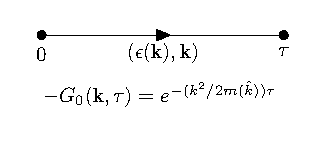
\includegraphics[scale=1.5]{free_el_propagator.pdf}
    \caption{Feynman diagram of the free electron propagator together with its Green's function.}
    \label{fig:el_prop_free}
\end{figure}
\begin{figure}[H]
    \centering
    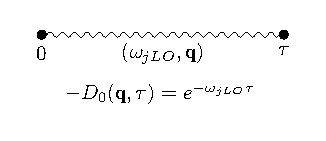
\includegraphics[scale=1.5]{free_ph_propagator.pdf}
    \caption{Feynman diagram of the free phonon propagator together with its Green's function.}
    \label{fig:ph_prop_free}
\end{figure}
In the same way, it is possible to find an explicit form for the phonon free propagator:
\begin{equation}
    D_0(\mathbf{q}j,\tau)=-\langle 0|a_\mathbf{q}(\tau)a^\dagger_\mathbf{q}|0\rangle=-e^{-\omega_{jLO}\tau},\hspace{1cm}\tau\ge0,
\end{equation}
which is again a simple exponential function.
\begin{figure}[H]
    \centering
    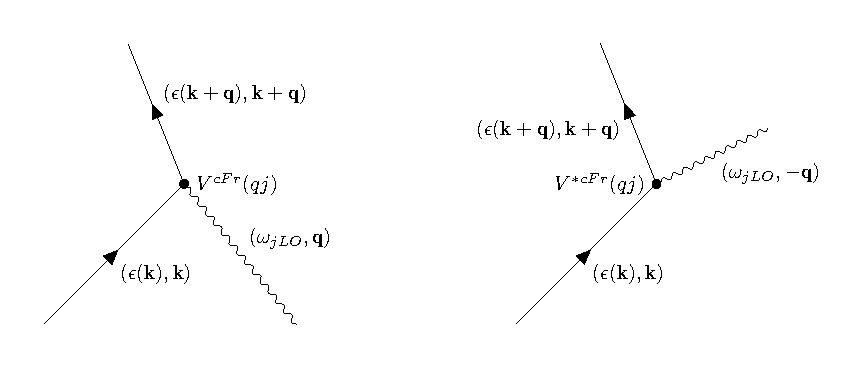
\includegraphics[scale=1.0]{interaction_vertex.pdf}
    \caption{Feynman diagrams of the electron-phonon interaction.}
    \label{fig:interaction_vertex}
\end{figure}
We now take into consideration the interaction part of the Froehlich Hamiltonian:
\begin{equation}
    V=\sum_{\mathbf{k},\mathbf{q}j}c^\dagger_{\mathbf{k+q}}c_{\mathbf{k}}\left[V^{cFr}_\mathbf{q}a_\mathbf{q}+V^{*cFr}_\mathbf{q}a^\dagger_\mathbf{-q}\right],
    \label{polaron_interacting}
\end{equation}
The basic Feynman diagram that describes this interaction is an interaction between two free electron propagators (one with momentum 
$\mathbf{k}$ gets annihilated and one with momentum $\mathbf{k+q}$ gets created) and a free phonon propagator which can either be annihilated (momentum 
$\mathbf{q}$) or created (momentum $\mathbf{-q}$), the strength of the interaction at the vertex is given by $|V_\mathbf{q}|$ (\ref{fig:interaction_vertex}).\\
We have now obtained the fundamental building blocks which can be used to obtain the total Green's function for the Froehlich polaron 
$G(\mathbf{k},\tau)$, a generic one-electron Matsubara Green's function for the polaron is written as \cite{mishchenko2000diagrammatic}
\begin{equation}
    G(\mathbf{k},\tau-\tau')= -\langle c_\mathbf{k}(\tau)c^\dagger_\mathbf{k}(\tau')\rangle =-\langle 0|c_\mathbf{k}(\tau)c^\dagger_\mathbf{k}(\tau')|0\rangle.
\end{equation}
The creation and annihilation operators here defined do not have the simple form described above for the free propagators, it is thus 
necessary to use the interaction picture and thus transform the operators:
\begin{equation}
    c_{I\mathbf{k}}(\tau)=e^{\tau H^{cFr}_0}c_{\mathbf{k}}e^{-\tau H^{cFr}_0},\hspace{1cm}c^\dagger_{I\mathbf{k}}(\tau)=e^{\tau H^{cFr}_0}c^\dagger_{\mathbf{k}}e^{-\tau H^{cFr}_0}.
\end{equation}
\begin{figure}[H]
    \centering
    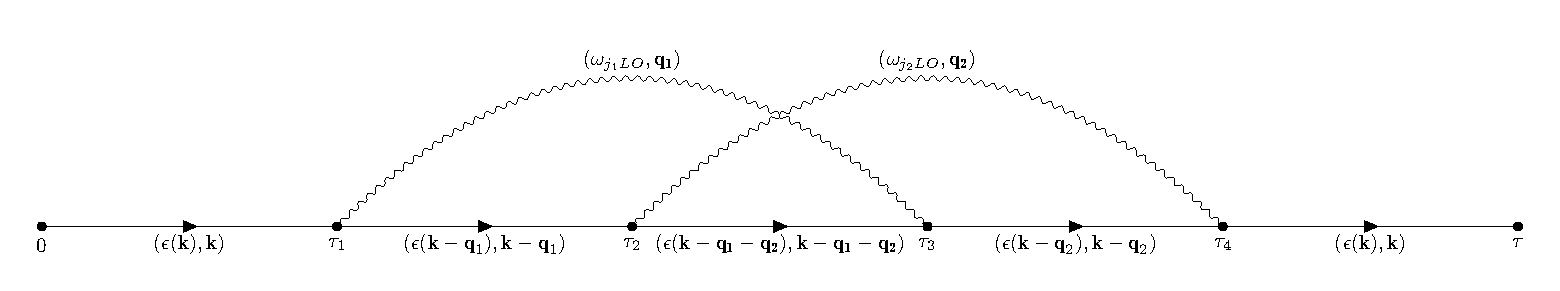
\includegraphics[scale=0.55]{diagram_order_4_2.pdf}
    \caption{Order 4 diagram.}
    \label{fig:diagram_order_4_2}
\end{figure}
\begin{figure}[H]
    \centering
    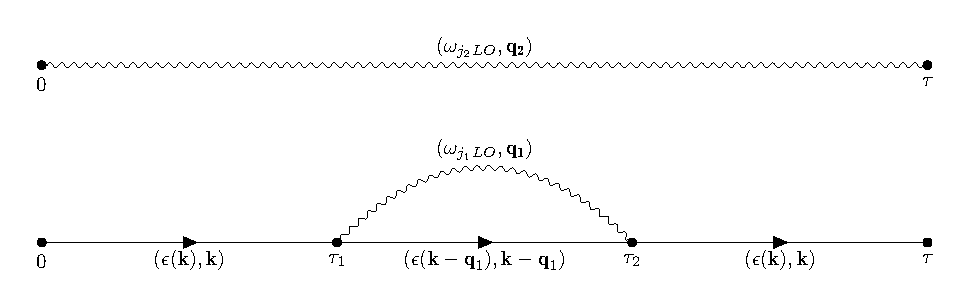
\includegraphics[scale=0.8]{diagram_disconnected.pdf}
    \caption{Disconnected order 4 diagram.}
    \label{fig:diagram_disconnected}
\end{figure}
In the interaction picture the Green's function for the Froehlich polaron assumes the form \cite{mishchenko2005diagrammatic}:
\begin{equation}
    G(\mathbf{k},\tau)=-\left\langle 0 \left| T_\tau\left[c_{I\mathbf{k}}(\tau)c^\dagger_\mathbf{k}\exp{\left(-\int_0^{+\infty}V_I(\tau')d\tau'\right)}\right]\right|0\right\rangle_{\text{conn}},
\end{equation}
where the expectation value is restricted to connected diagrams, which means that no integral over the internal variables $d\tau_i'$ can be represented 
by an external factor (the difference between a connected and disconnected diagram is easily recognazible in \ref{fig:diagram_order_4_2} and 
\ref{fig:diagram_disconnected}).
\begin{figure}[H]
    \centering
    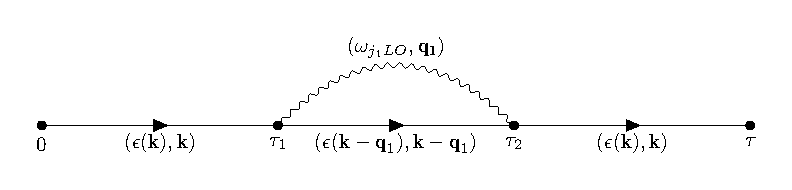
\includegraphics[scale=0.745]{diagram_order_2.pdf}
    \caption{Order 2 diagram.}
    \label{fig:diagram_order_2}
\end{figure}
\begin{figure}[H]
    \centering
    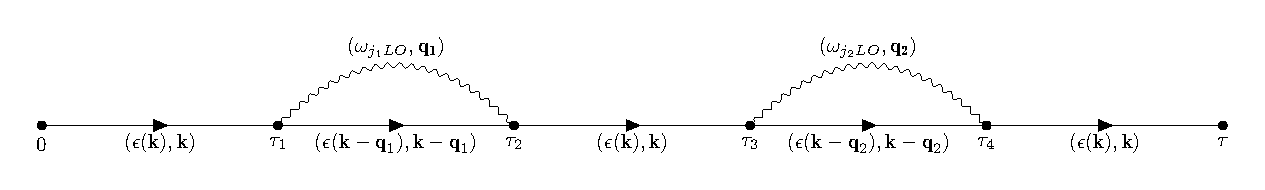
\includegraphics[scale=0.738]{diagram_order_4_1.pdf}
    \caption{Order 4 diagram.}
    \label{fig:diagram_order_4_1}
\end{figure}
\begin{figure}[H]
    \centering
    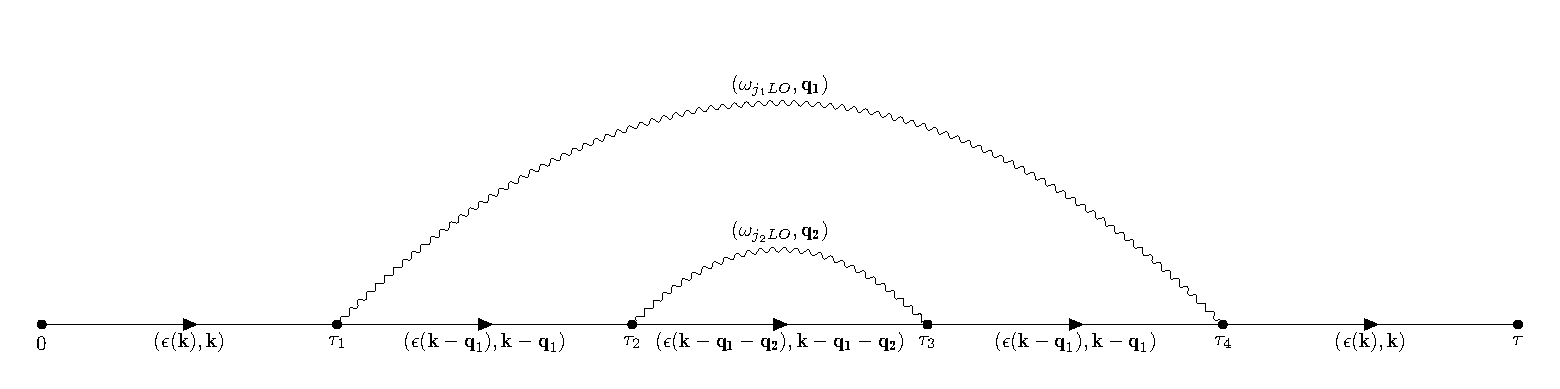
\includegraphics[scale=0.58]{diagram_order_4_3.pdf}
    \caption{Order 4 diagram.}
    \label{fig:diagram_order_4_3}
\end{figure}
Using Wick's theorem, the product of $n$ chronologically ordered operators $\{\tau_1,\tau_2,...,\tau_n\}$ can be evaluated as the sum 
of products of pairs of operators, such that it is possible to expand the Green's function as an infinite series of terms of the following form:
\begin{equation}
    G(\mathbf{k},\tau)=-\sum_{n=0,2,4...}^{+\infty}\sum_{\xi_n}\int d\tau_1\cdots\int d\tau_n D_n^{\xi_n}(\mathbf{k},\tau;x_1,...,x_n),
    \label{GF_polaron_series}
\end{equation}
where $n$ indexes the rank of the term (only terms with an even number of internal variables are allowed), $\xi_n$ indexes the topology of the 
term (which depends on how the phonon lines are arranged, see the difference between \ref{fig:diagram_order_4_1}, \ref{fig:diagram_order_4_2} and 
\ref{fig:diagram_order_4_3}), $x_i$ are the internal variables which index the imaginary times at which a vertex $V^{cFr}(qj)$ is 
present (and a phonon is created or annihilated), the index $j$ of the phonon mode which interacts with the electron propagators and the momentum $q$ of the created/annihilated 
phonon line.\\
As an example, the 0-order term is just the free electron propagator $G_0(\mathbf{k},\tau)=-e^{-\epsilon(\mathbf{k})\tau}$, the 2-order term 
(with internal variables $(\tau_1,j_1)$ and $(\tau_2,j_2)$) represents a diagram with 3 free electron propagators, 1 free phonon propagator and 2 vertices.\\
$D_2(\mathbf{k},\tau;x_1,x_2,)$ can thus be represented using Green's function as
\begin{equation}
\begin{split}
    D_2(\mathbf{k},\tau;x_1,x_2,)=&|V^{cFr}(qj)|^2D_0(\mathbf{q}j,\tau_2-\tau_1)G_0(\mathbf{k},\tau-\tau_2)\times\\
    &G_0(\mathbf{k-q},\tau_2-\tau_1)G_0(\mathbf{k},\tau_1),
\end{split}
\end{equation}
which translates to
\begin{equation}
    D_2(\mathbf{k},\tau;x_1,x_2,)=|V^{cFr}(qj)|^2e^{-\omega_{jLO}(\tau_2-\tau_1)}e^{-\epsilon(\mathbf{k})(\tau-\tau_2)}e^{-\epsilon(\mathbf{k-q})(\tau_2-\tau_1)}e^{-\epsilon(\mathbf{k})\tau_1}.
\end{equation}
It should be noted that in our computation instead of \ref{GF_polaron_series} the result without the minus sign will be taken: this is just a convention 
used in order to obtain a definite positive distribution for the Monte Carlo sampling and it does not affect the physical significance of the calculated Green's functions.\\
Having seen the one-electron Green's function we now introduce another related Green's function: the one-electron $N$-phonons Green's function 
$G^N(\mathbf{k},\sum_{j=1}^N\mathbf{\tilde{q}}_j,\tau)$. Differently from the one-elecron Green's function, the one-electron $N$-phonons Green's function is a more complex object consisting of 
$N$ phonons and one electron, and better describes the polaron physics, expecially if the strength of the interaction is intense.\\
Its expression, using Wick's theorem, can be written as \cite{hahn2018diagrammatic}:
\begin{equation}
    G^N(\mathbf{k},\sum_{j=1}^N\mathbf{\tilde{q}}_j,\tau)=\left\langle 0|a_{\mathbf{\tilde{q}}_1}(\tau)...a_{\mathbf{\tilde{q}}_N}(\tau)c_{\mathbf{p}}(\tau)c^\dagger_{\mathbf{p}}a_{\mathbf{\tilde{q}}_N}...a_{\mathbf{\tilde{q}}_1} |0\right\rangle,
\end{equation}
where $\mathbf{p}=\mathbf{k}-\sum_{j=1}^N\mathbf{\tilde{q}}_j$.\\
It is worth noting that $G^N(\mathbf{k},\sum_{j=1}^N\mathbf{\tilde{q}},\tau)$ will only take into account connected one-electron $N$-phonons Green's functions since in the other cases the external 
phonons can just be neglected. The related expansion can be given as:
\begin{equation}
\begin{split}
        G^N(\mathbf{k},\sum_{j=1}^N\mathbf{\tilde{q}}_j,\tau)=&\sum_{n=0,2,4...}^{+\infty}\sum_{\xi_n}\int d\mathbf{\tilde{q}}_1\cdots \int d\mathbf{\tilde{q}}_N \cdot \\
         &\cdot\int d\tau_1\cdots\int d\tau_n D_n^{\xi_n}(\mathbf{k},\sum_j\mathbf{\tilde{q}}_j,\tau;x_1,...,x_n),
\end{split}
\label{GF_N_polaron_series}
\end{equation}
where the minus sign has been dropped.
\begin{figure}[H]
    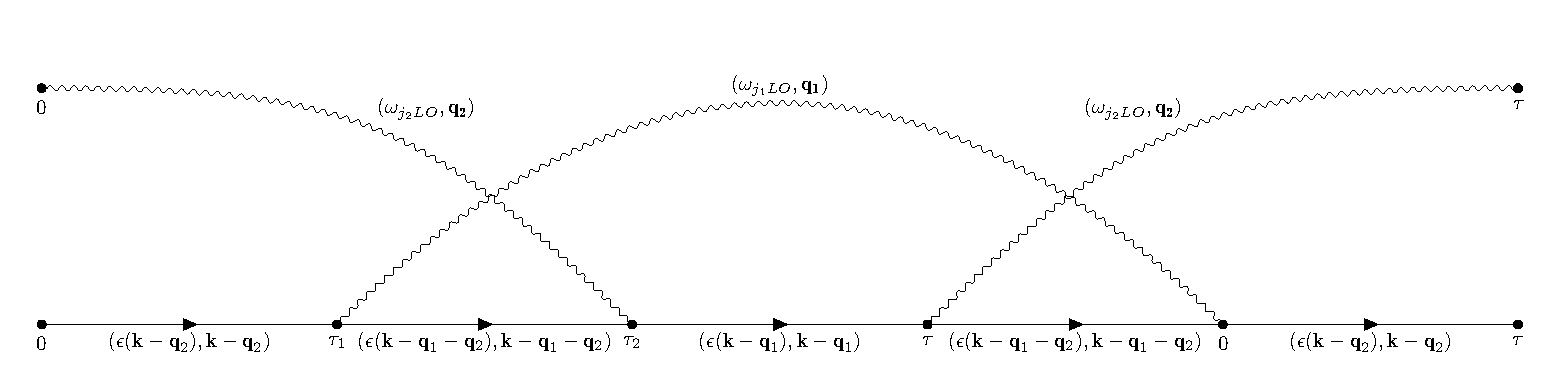
\includegraphics[scale = 0.55]{diagram_order_2_N2.pdf}
    \caption{Order 2 diagram with one external phonon.}
    \label{fig:diagram_order_2_N2}
\end{figure}
It is thus useful to consider the full function $P(\mathbf{k},\tau)$ defined as follows:
\begin{equation}
    P(\mathbf{k},\tau)=G(\mathbf{k},\tau)+\sum_{N=1}^{+\infty}G^N(\mathbf{k},\sum_{j=1}^N\mathbf{\tilde{q}}_j,\tau),
\end{equation}
which more accurately describes our polaron model, including both the "free" polaron and its interaction with the phonon cloud.

